%!TeX root = ../report.tex


\chapter{Annexos}
\label{ch:annexos}

\section{Captures de pantalla de la interfície}
\label{sec:annex-screenshots}

Aquest annex recull totes les captures de pantalla referenciades al capítol de Disseny (\autoref{ch:disseny}), agrupades
per àrea funcional de la interfície.

\subsection{Pantalla d'inici}
\label{subsec:annex-landing}

\begin{figure}[ht]
    \centering
    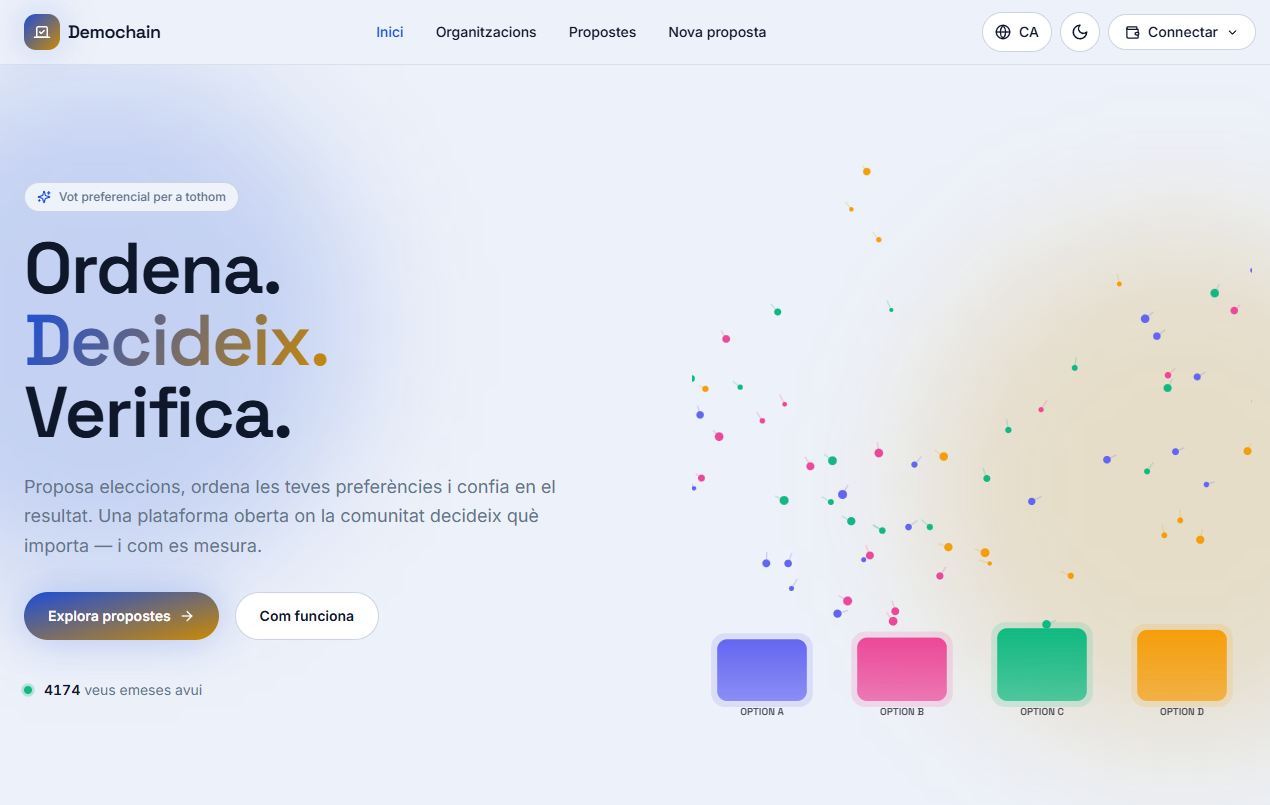
\includegraphics[width=\textwidth]{chapters/images/disseny/screenshots/01-landing}
    \caption{Pantalla d'inici de DemoChain. Capçalera de navegació, selector d'idioma i connexió de cartera.}
    \label{fig:ui-landing}
\end{figure}

\subsection{Gestió d'organitzacions}
\label{subsec:annex-organizations}

\begin{figure}[ht]
    \centering
    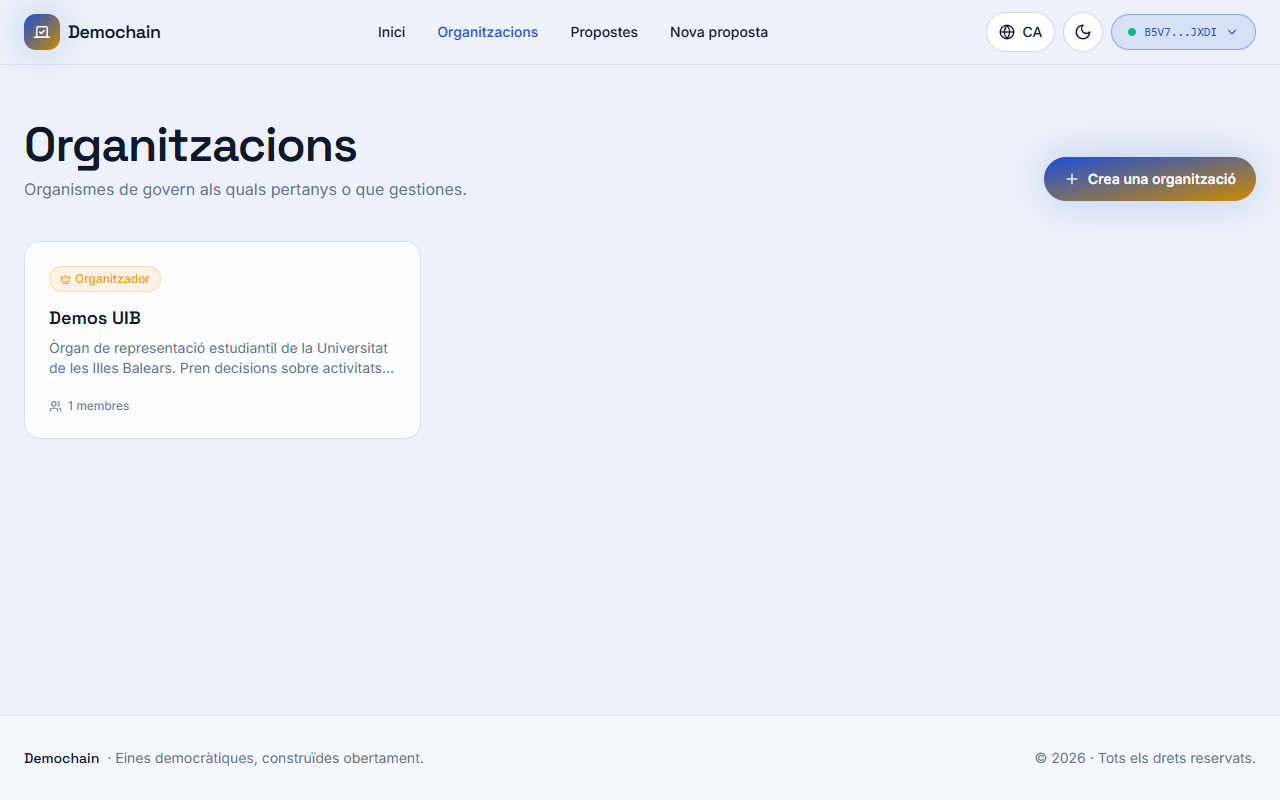
\includegraphics[width=\textwidth]{chapters/images/disseny/screenshots/02-organizations}
    \caption{Llistat d'organitzacions a què pertany el votant connectat.}
    \label{fig:ui-organizations}
\end{figure}

\begin{figure}[ht]
    \centering
    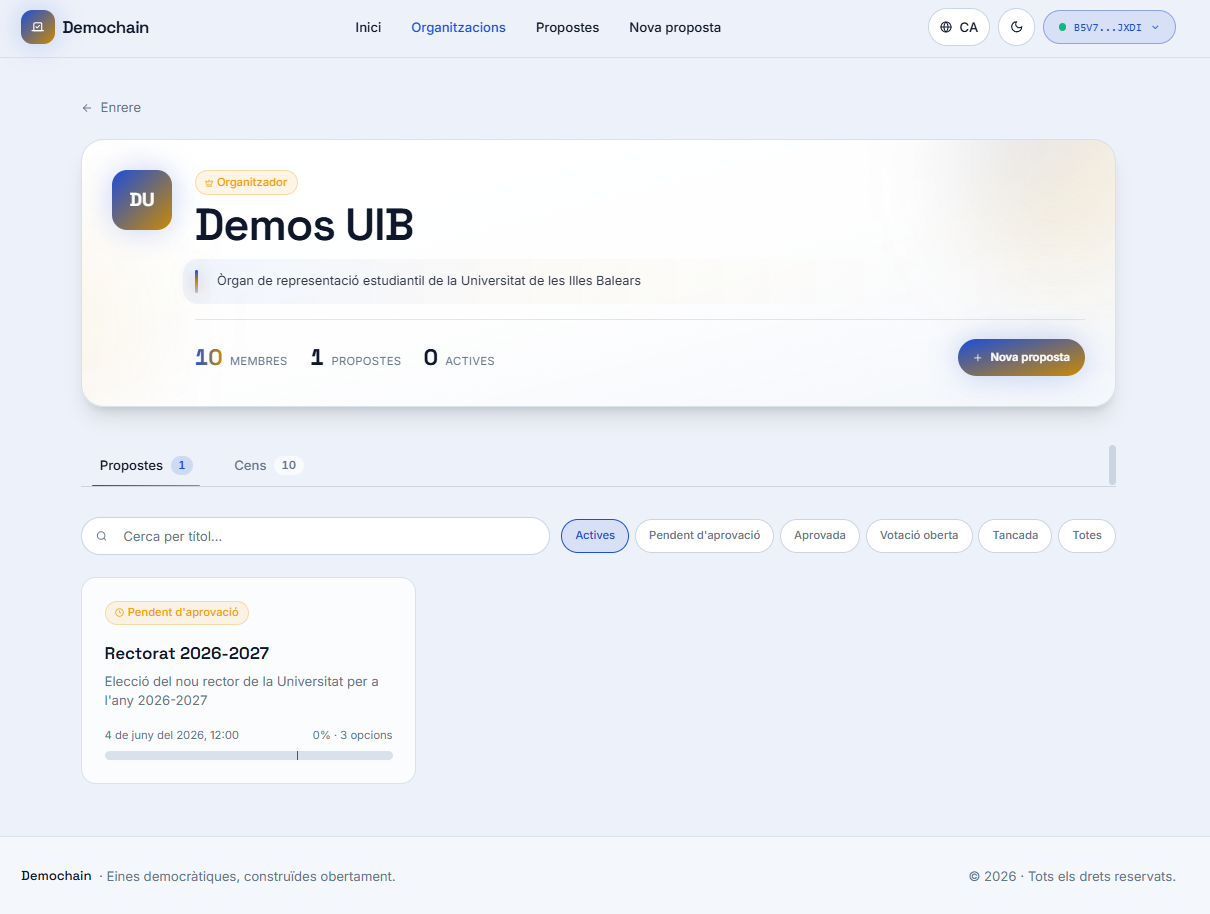
\includegraphics[width=\textwidth]{chapters/images/disseny/screenshots/03-organization-detail}
    \caption{Detall d'una organització, amb pestanyes de propostes i cens. L'organització té una proposta activa, encara sense vots d'aprovació.}
    \label{fig:ui-organization-detail}
\end{figure}

\subsection{Propostes}
\label{subsec:annex-proposals}

\begin{figure}[ht]
    \centering
    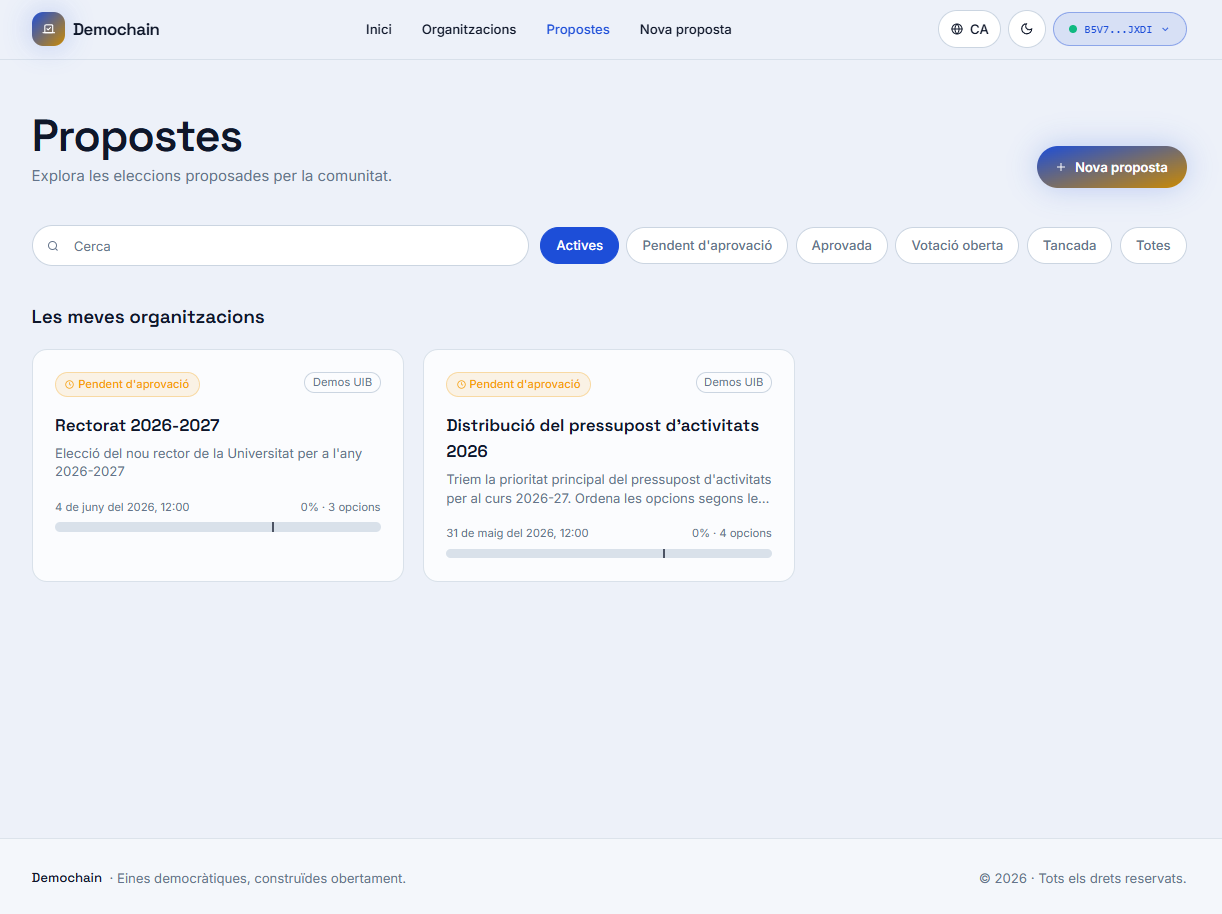
\includegraphics[width=\textwidth]{chapters/images/disseny/screenshots/04-proposals-list}
    \caption{Llistat de propostes amb filtres per estat. L'usuari que veu aquesta pantalla té dues propostes que estan \textit{pendents d'aprovació} de l'organització \textit{``Demos UIB''} (organització a la que pertany).}
    \label{fig:ui-proposals-list}
\end{figure}

\begin{figure}[ht]
    \centering
    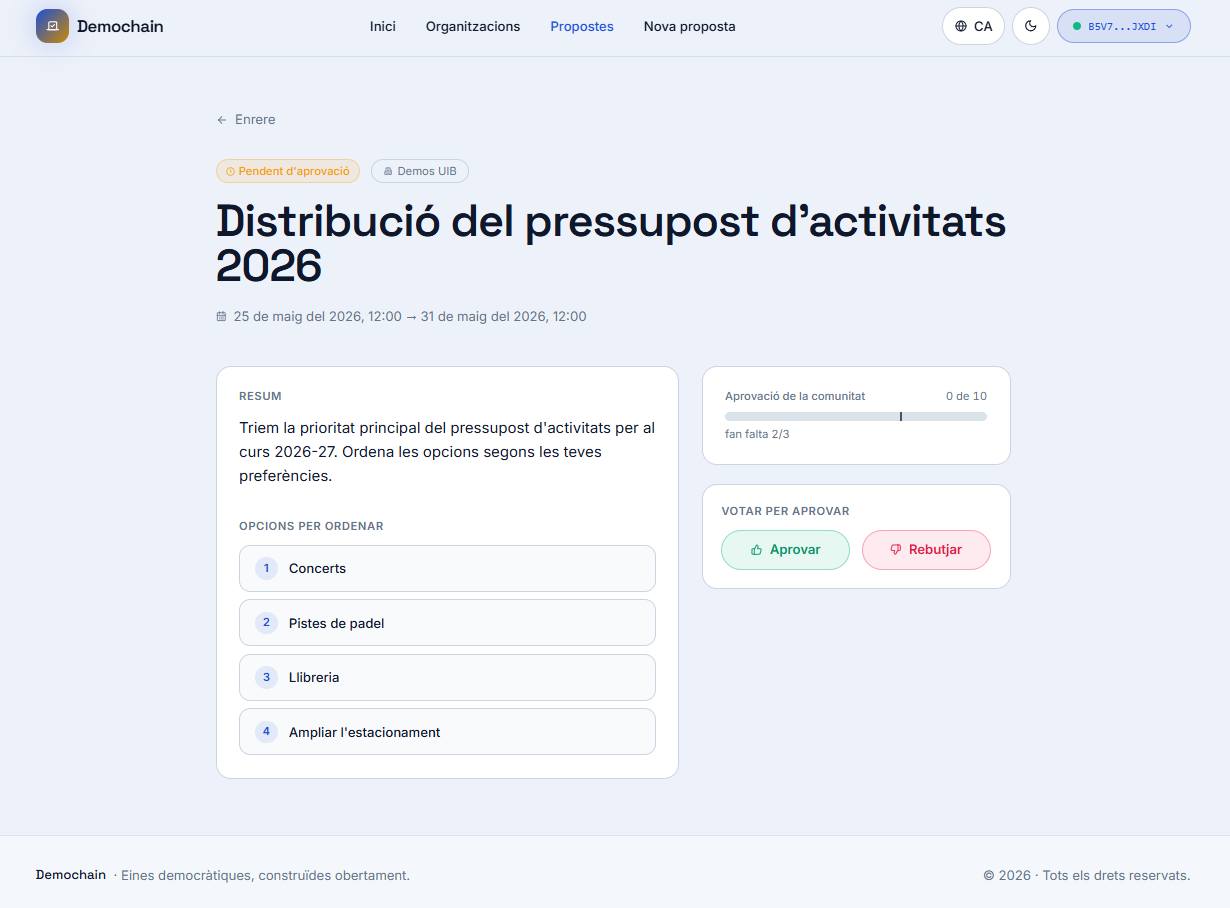
\includegraphics[width=\textwidth]{chapters/images/disseny/screenshots/04b-proposal}
    \caption{Informació concreta d'una proposta: títol, resum, opcions, recompte de vots i formulari per aprobar o rebutjar la proposta.}
    \label{fig:ui-proposal}
\end{figure}

\begin{figure}[ht]
    \centering
    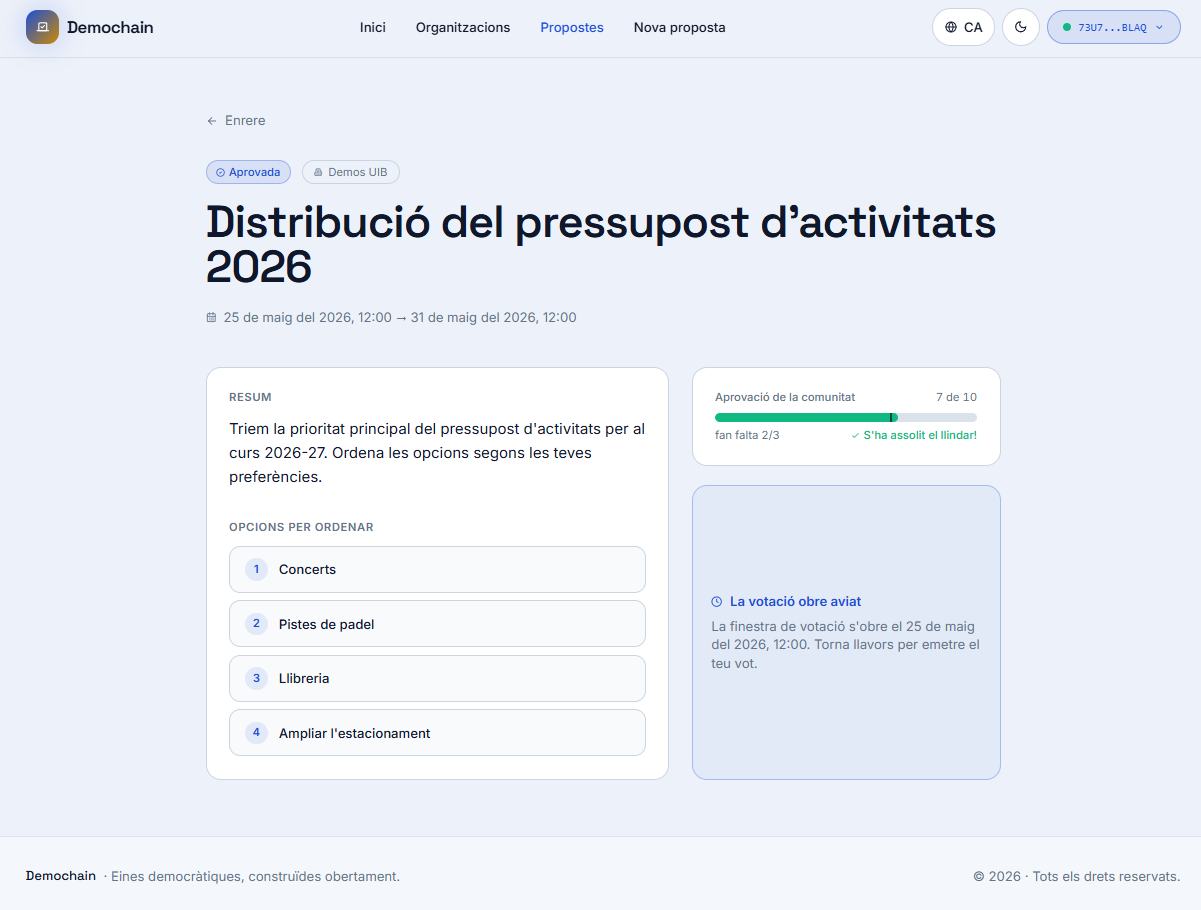
\includegraphics[width=\textwidth]{chapters/images/disseny/screenshots/04c-proposal}
    \caption{Informació concreta d'una proposta que s'ha aprovat i encara no ha començat el període de votació.}
    \label{fig:ui-proposal-aproved}
\end{figure}

\subsection{Creació d'una proposta}
\label{subsec:annex-new-proposal}

\begin{figure}[ht]
    \centering
    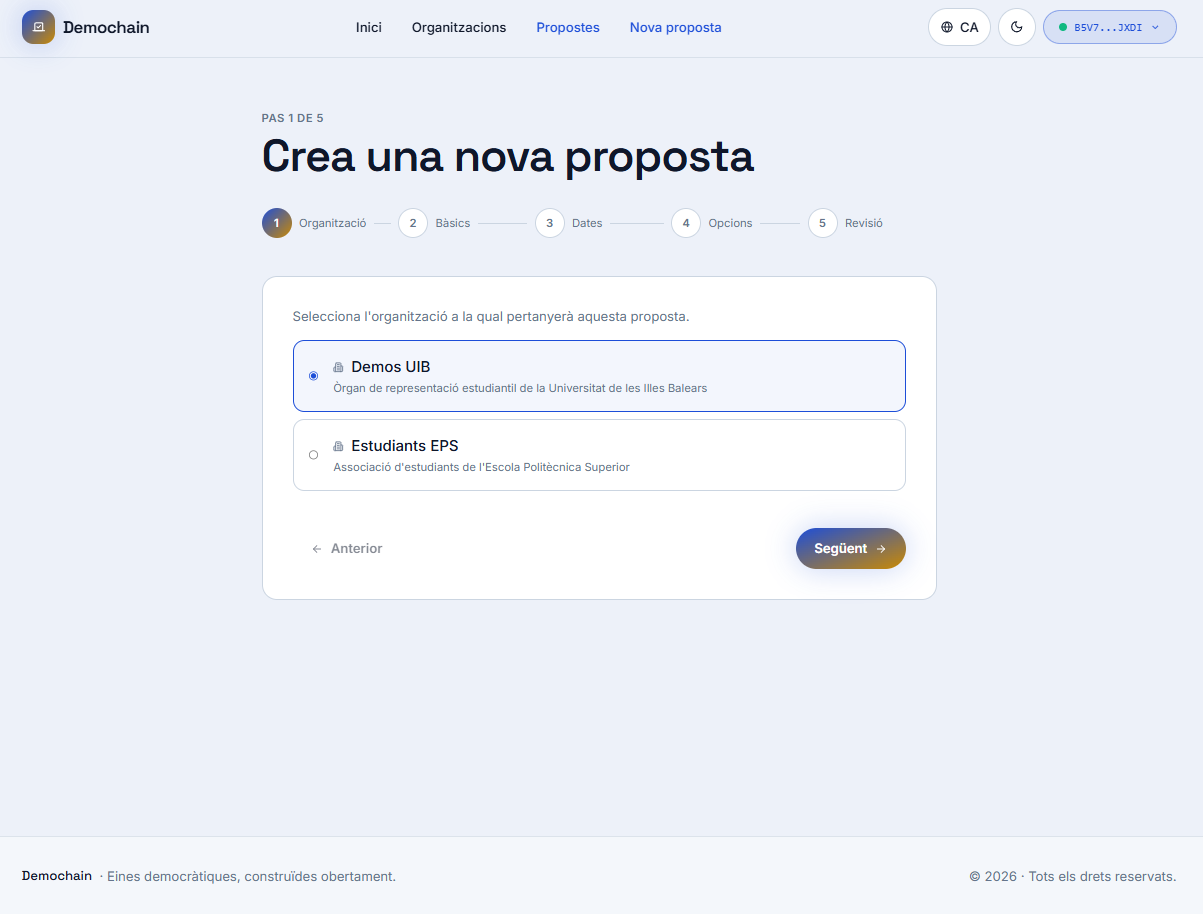
\includegraphics[width=\textwidth]{chapters/images/disseny/screenshots/05-new-proposal-1}
    \caption{Assistent de creació d'una proposta, pas \textit{Organització}.}
    \label{fig:ui-new-proposal-1}
\end{figure}

\begin{figure}[ht]
    \centering
    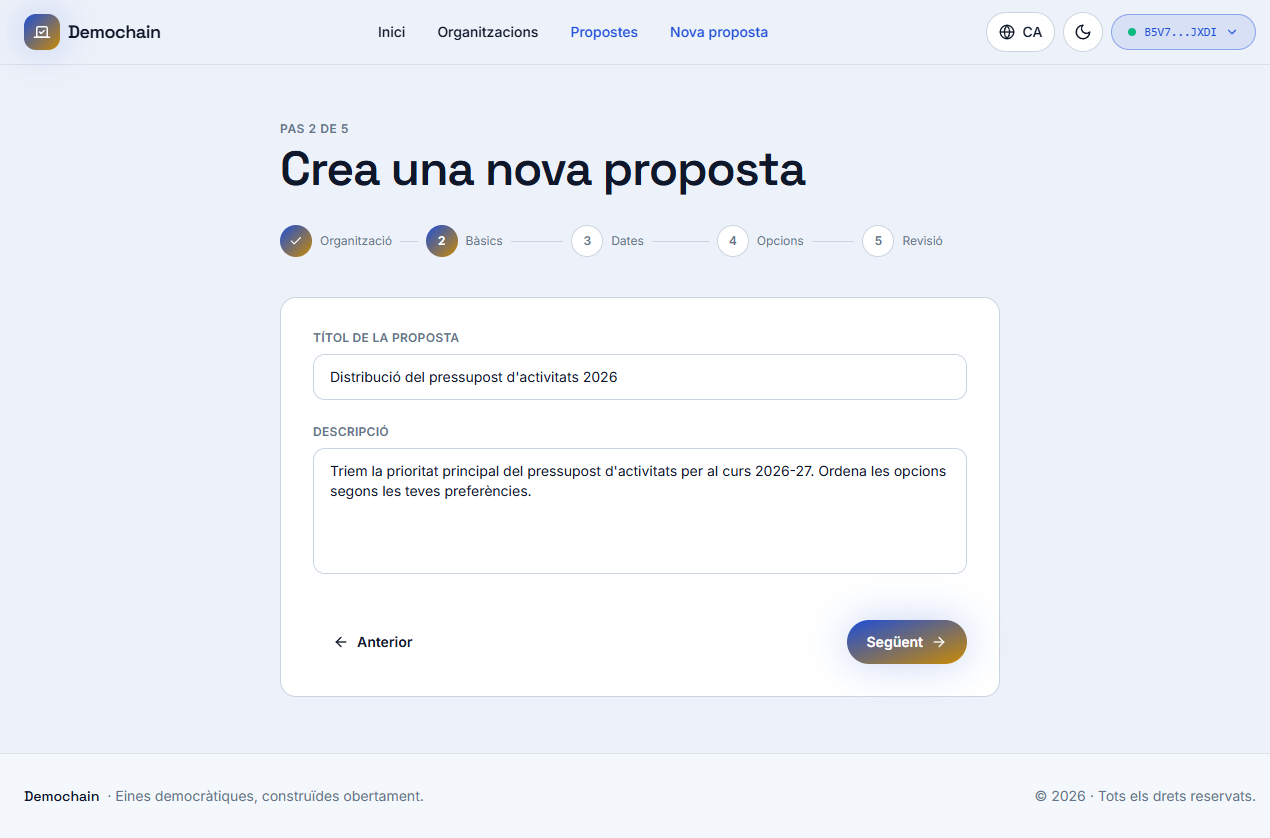
\includegraphics[width=\textwidth]{chapters/images/disseny/screenshots/05-new-proposal-2}
    \caption{Assistent de creació d'una proposta, pas \textit{Bàsics}.}
    \label{fig:ui-new-proposal-2}
\end{figure}

\begin{figure}[ht]
    \centering
    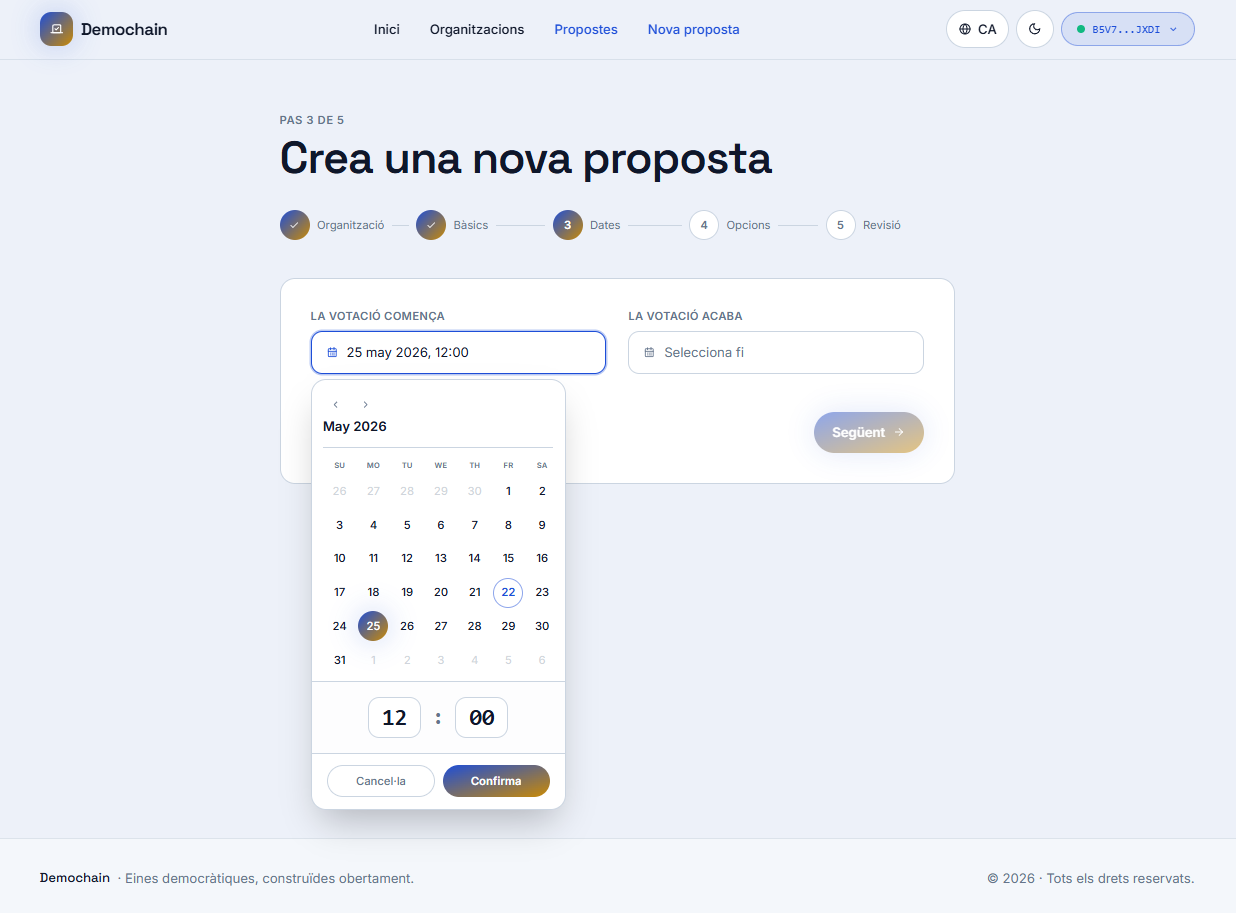
\includegraphics[width=\textwidth]{chapters/images/disseny/screenshots/05-new-proposal-3}
    \caption{Assistent de creació d'una proposta, pas \textit{Dates}.}
    \label{fig:ui-new-proposal-3}
\end{figure}

\begin{figure}[ht]
    \centering
    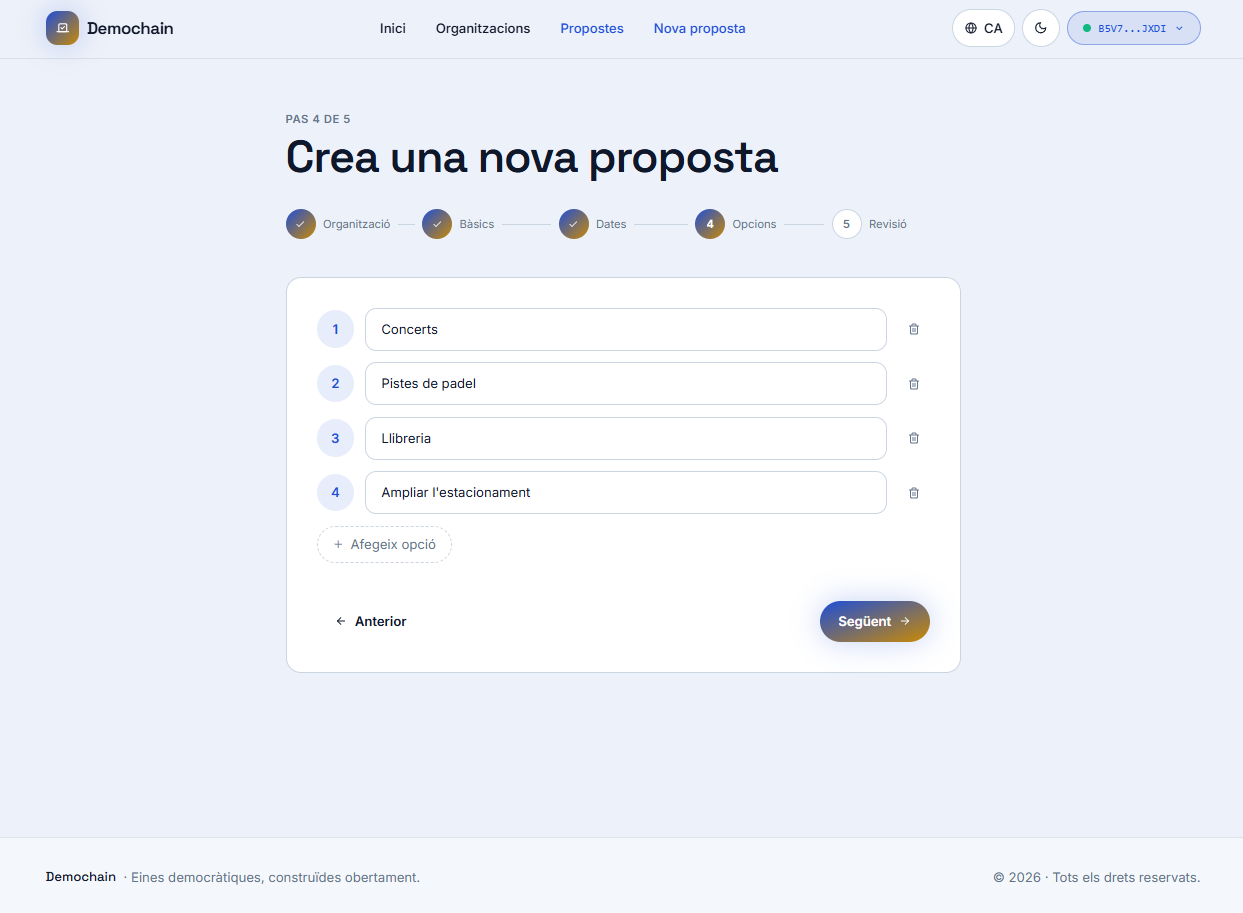
\includegraphics[width=\textwidth]{chapters/images/disseny/screenshots/05-new-proposal-4}
    \caption{Assistent de creació d'una proposta, pas \textit{Opcions}.}
    \label{fig:ui-new-proposal-4}
\end{figure}

\begin{figure}[ht]
    \centering
    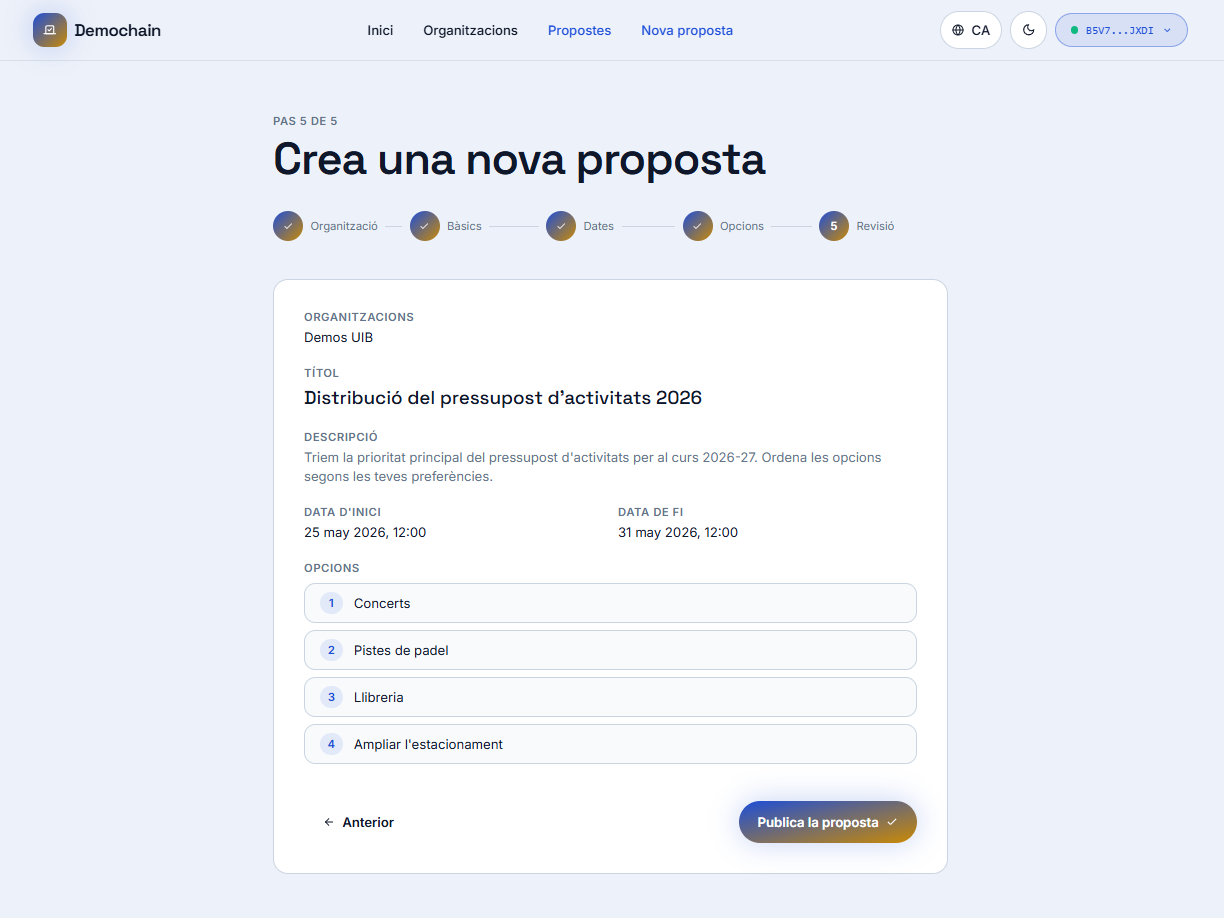
\includegraphics[width=\textwidth]{chapters/images/disseny/screenshots/05-new-proposal-5}
    \caption{Assistent de creació d'una proposta, pas \textit{Revisió}.}
    \label{fig:ui-new-proposal-5}
\end{figure}

\subsection{Emissió de vot}
\label{subsec:annex-vote}

\begin{figure}[ht]
    \centering
    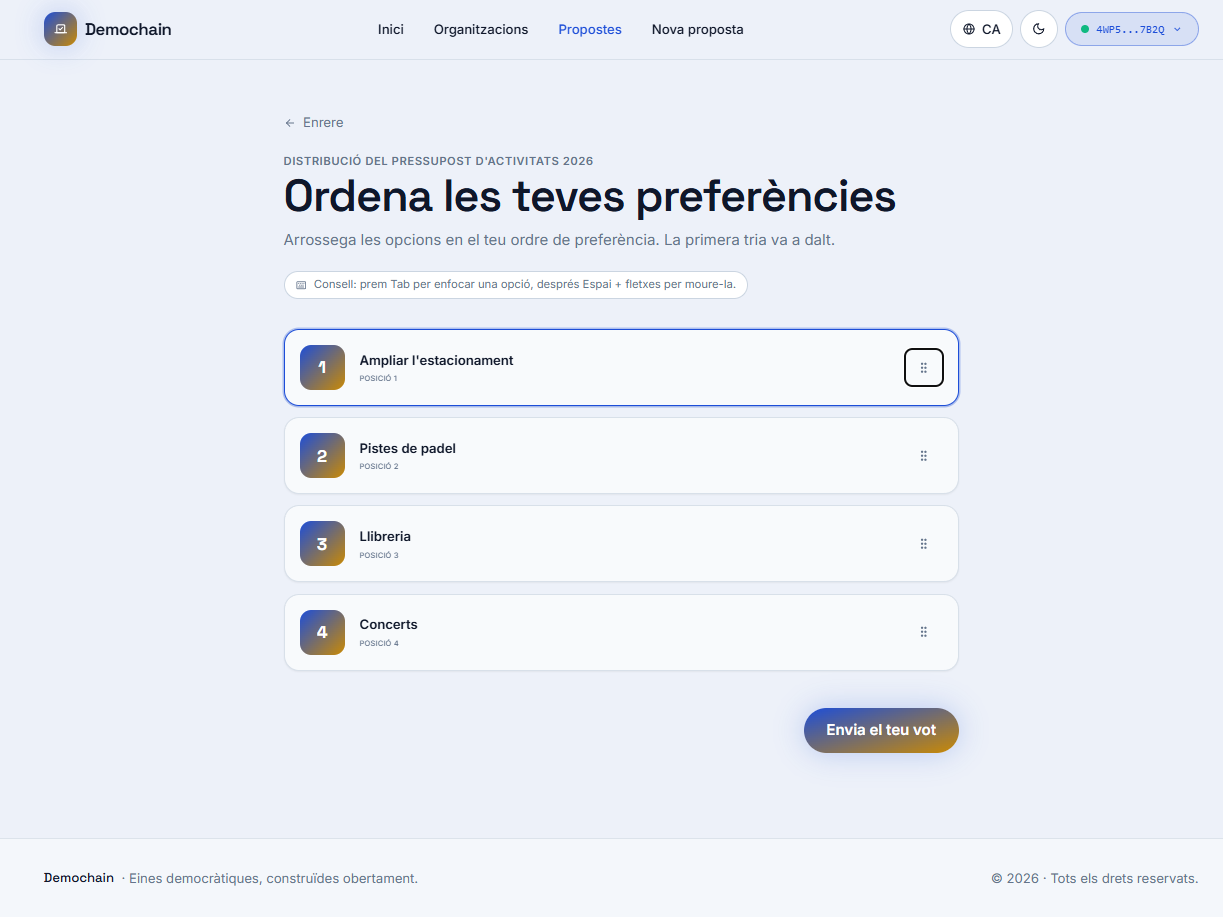
\includegraphics[width=\textwidth]{chapters/images/disseny/screenshots/06-vote-ranking}
    \caption{Pantalla d'emissió de vot: ranking de preferències arrossegables.}
    \label{fig:ui-vote}
\end{figure}

\begin{figure}[ht]
    \centering
    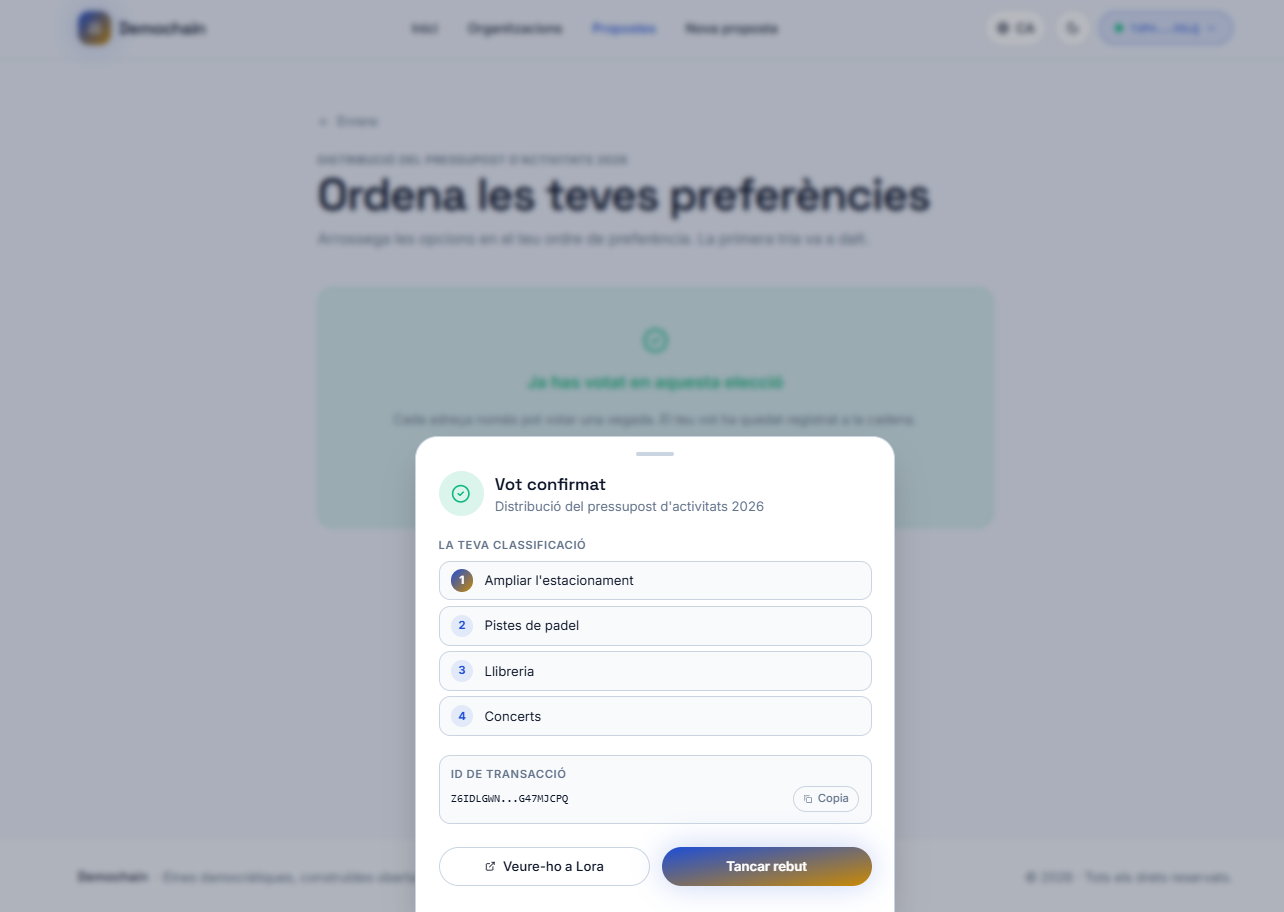
\includegraphics[width=\textwidth]{chapters/images/disseny/screenshots/06b-vote-ranking}
    \caption{Pantalla dde vot confirmat.}
    \label{fig:ui-vote-confirm}
\end{figure}

\begin{figure}[ht]
    \centering
    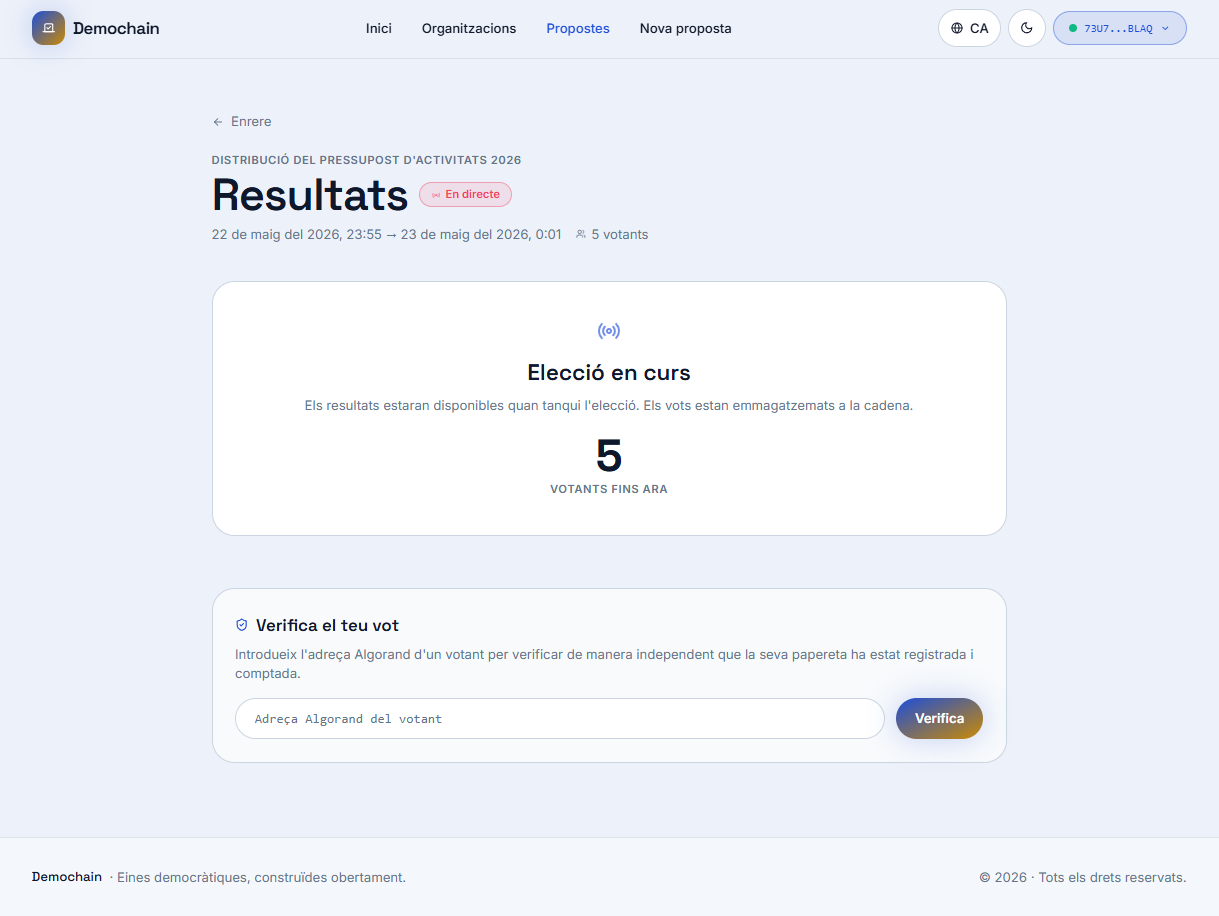
\includegraphics[width=\textwidth]{chapters/images/disseny/screenshots/06c-vote-ranking}
    \caption{Pantalla de seguiment d'enviament de vots}
    \label{fig:ui-vote-num}
\end{figure}

\subsection{Resultats i verificació pública}
\label{subsec:annex-results}

\begin{figure}[ht]
    \centering
    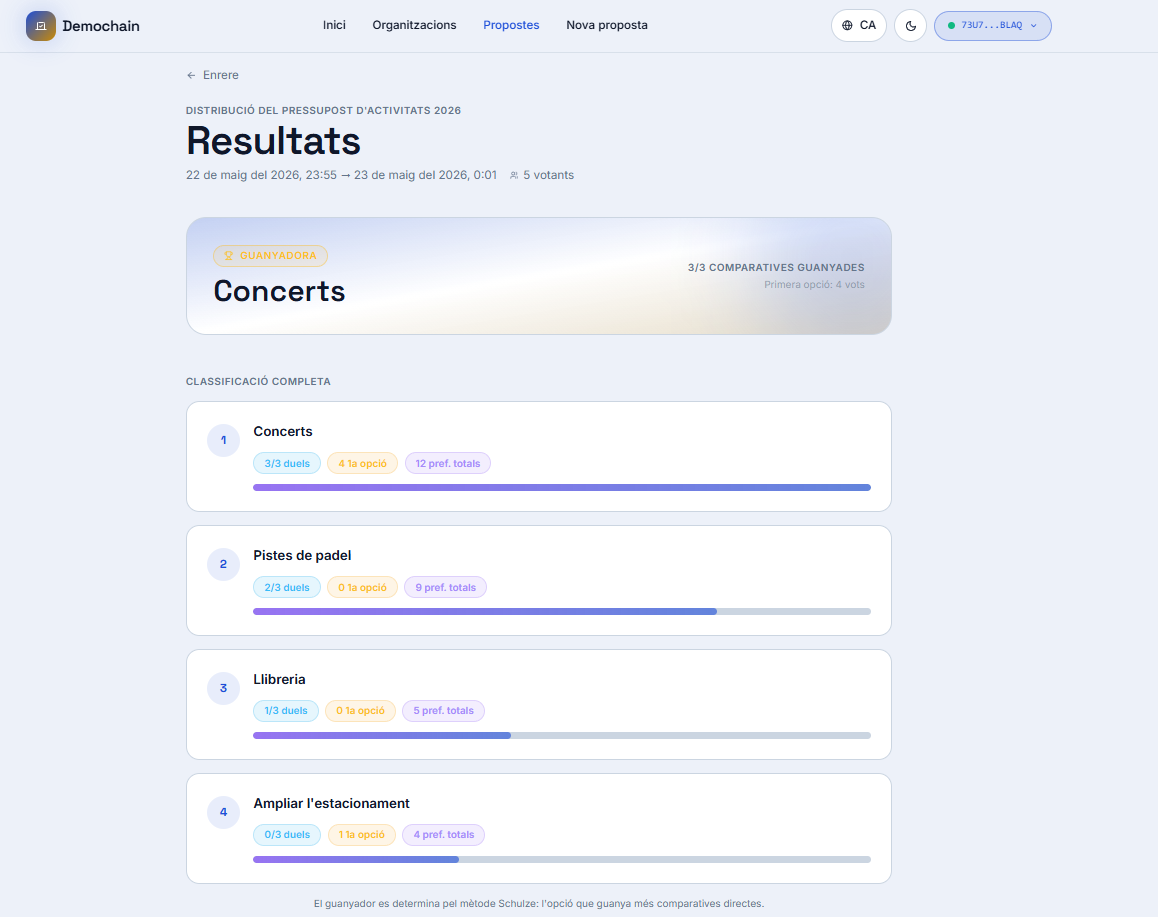
\includegraphics[width=\textwidth]{chapters/images/disseny/screenshots/07-results}
    \caption{Pantalla de resultats finals i verificació pública.}
    \label{fig:ui-results-1}
\end{figure}

\begin{figure}[ht]
    \centering
    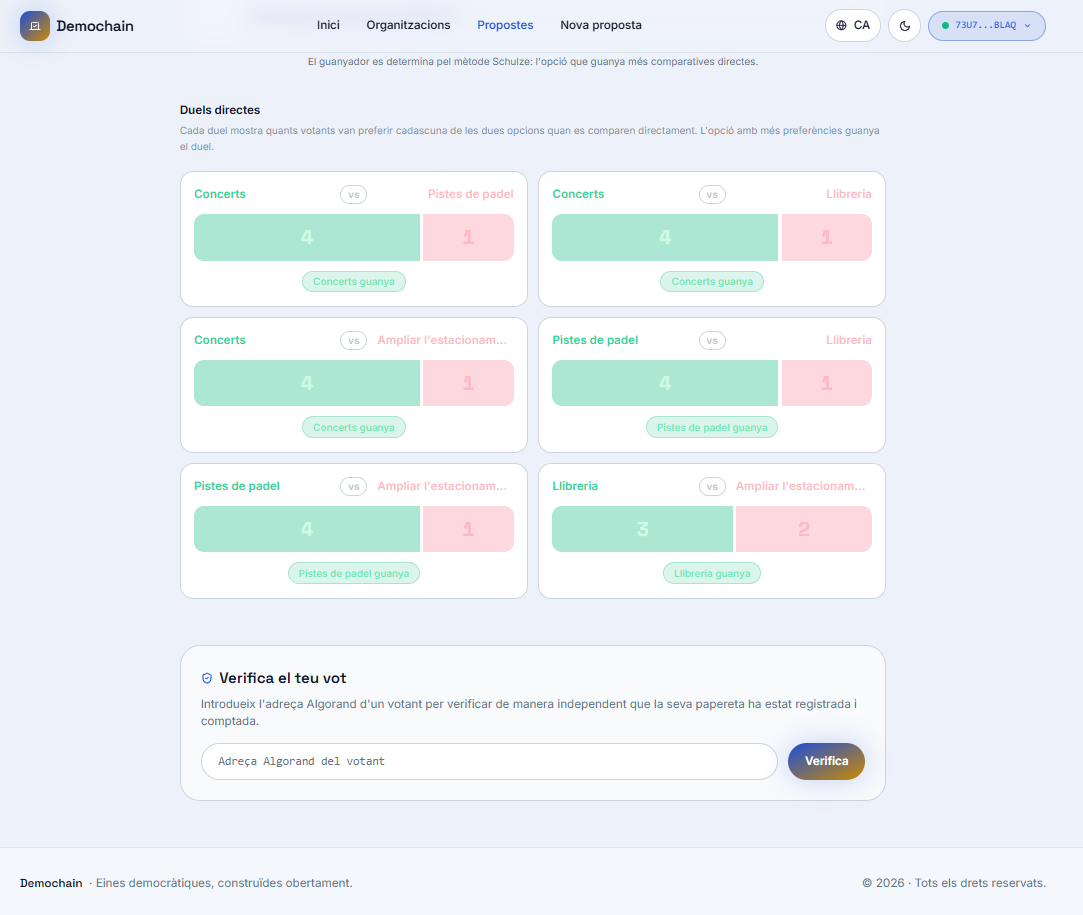
\includegraphics[width=\textwidth]{chapters/images/disseny/screenshots/07b-results}
    \caption{Pantalla de resultats amb els duels directes.}
    \label{fig:ui-results-2}
\end{figure}

\begin{figure}[ht]
    \centering
    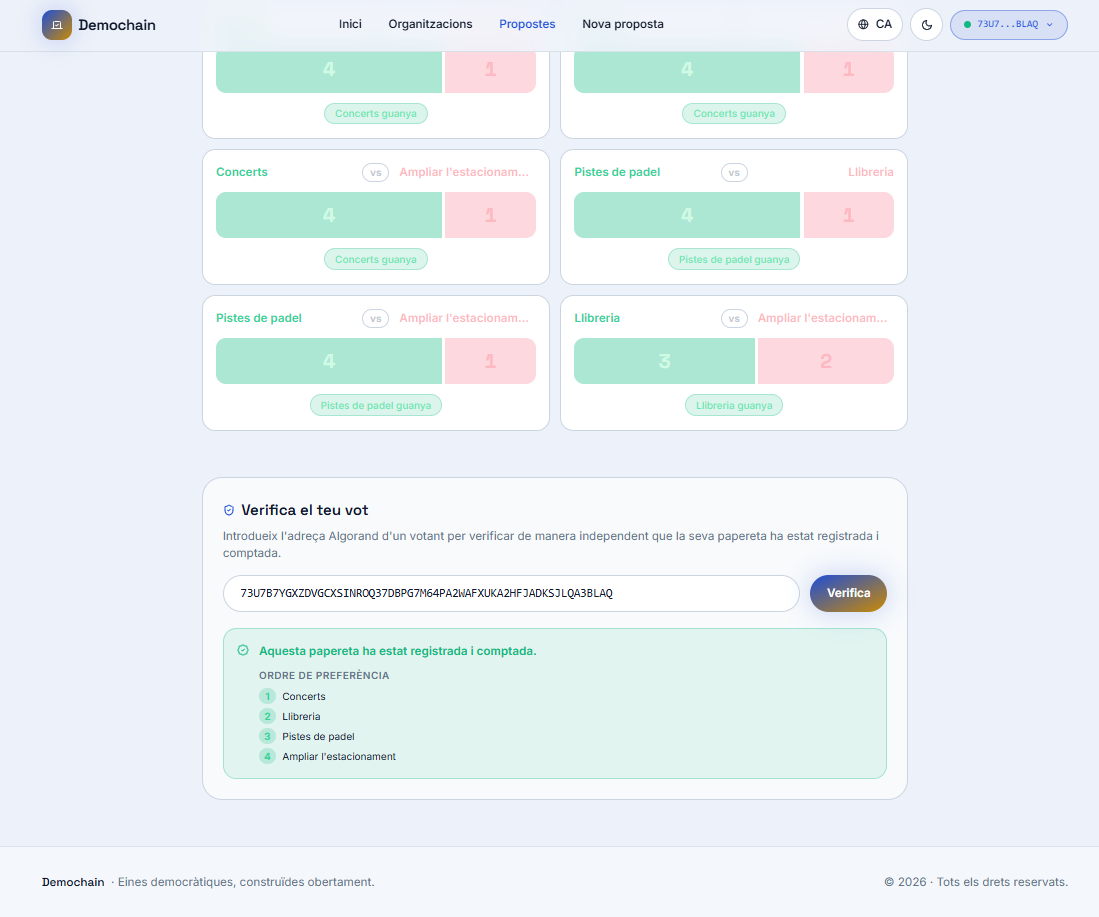
\includegraphics[width=\textwidth]{chapters/images/disseny/screenshots/07c-results}
    \caption{Pantalla de verificació del vot que s'ha emès una vegada acabada l'elecció.}
    \label{fig:ui-results-3}
\end{figure}
